\subsection{Overview}
Different from uninformed search and informed search. 
\begin{outline}
    \1 Uninformed search
        \2 use only information on \textbf{current path}, that is, from goal to fringe
    \1 Informed search
        \2 use also \textbf{heuristics}, that is, information about how close nodes on the fringe are to a goal
\end{outline}

\noindent
A heuristics is a function that estimates \textbf{how close a state is to a goal}, which needs \textbf{domain knowledge} \\

There is different heuristic function: manhattan distance, euclidean distance, ....

\subsection{Greedy search}
The difference between greedy search and uniformed search is \textbf{SELECT = "priority queue, order elements by $h(n)$}, which is called "Best-first search". \\
The difference between greedy search and uniformed cost-sensitive search is:
\begin{outline}
    \1 Greedy Search uses heuristic to order.
    \1 UCS uses accumulated cost to order.
\end{outline}

\noindent
Is it optimal? No, it just takes \textbf{the most obvious result} as next step, but may not be the best one. (Short-term vs. Long-term) Thus, the properties of greedy search is: (Time and space complexity is just badly-guide DFS)
\begin{outline}
    \1 Time complexity: $O(b^{m})$
        \2 with b: branching factor, m: maximum depth
    \1 Space complexity: $O(b^{m})$
        \2 with b: branching factor, m: maximum depth
    \1 Completeness: \textcolor{red}{no}, like badly DFS
    \1 Optimal: \textcolor{red}{no}, it just choose the most obvious result instead of the optimal one
\end{outline}

\subsection{Beam search}
A variant of \st{greedy search} and breadth-first search. It is similar to breadth-first, but only expend \emph{k} times \textbf{each tier}. First build the whole tier, then keep \emph{k} elements in frontier. The properties of beam search is:
\begin{outline}
    \1 Time complexity: \textcolor{red}{$O(k \times b \times s)$}
        \2 with k: hyperparameter, b: branching factor, s: shallowest-solution depth
    \1 Space complexity: \textcolor{red}{$O(k \times b)$}
        \2 with k: hyperparameter, s: shallowest-solution depth
    \1 Completeness: no, may drop the goal
    \1 Optimal: no, not completeness not even optimal
\end{outline}

\noindent
When k = 1, it is called \textbf{"Hill-Climbing search"}. \\

\subsection{Combination of UCS and Greedy Search}
As we known, UCS uses \textbf{path cost = "Backward cost" = $g(n)$} (Figure~\ref{fig:usc_path_cost}), and Greedy search uses \textbf{heuristic = "Forward cost = $h(n)$} (Figure~\ref{fig:greedy_search_heuristic}). And if we combine those two cost to estimate the quality of our current state: $f(n) = g(n) + h(n)$. The \textbf{SELECT = "priority queue, order elements by $f(n)$"} \\

\begin{figure}[htbp]
    \centering
    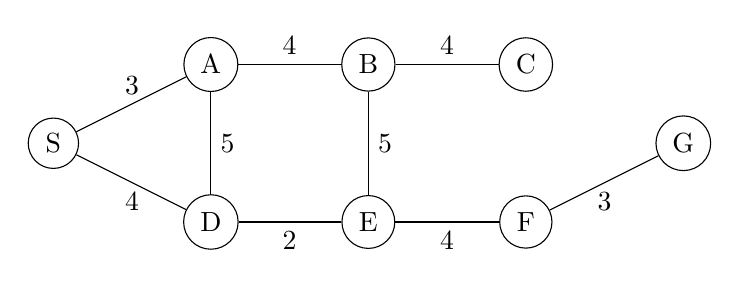
\begin{tikzpicture}
        \node [draw,circle](s)at(0,0){S};
        \node [draw,circle](a)at(2,1){A};
        \node [draw,circle](d)at(2,-1){D};
        \node [draw,circle](b)at(4,1){B};
        \node [draw,circle](e)at(4,-1){E};
        \node [draw,circle](c)at(6,1){C};
        \node [draw,circle](f)at(6,-1){F};
        \node [draw,circle](g)at(8,0){G};

        \draw (s) -- (a); 
        \draw (a) -- (b);
        \draw (b) -- (c);
        \draw (a) -- (d);
        \draw (s) -- (d);
        \draw (d) -- (e);
        \draw (b) -- (e);
        \draw (e) -- (f);
        \draw (f) -- (g);        

        \draw (1,1/2) node[above]{$3$};
        \draw (1,-1/2) node[below]{$4$};
        \draw (2,0) node[right]{$5$};
        \draw (3,1) node[above]{$4$};
        \draw (3,-1) node[below]{$2$};
        \draw (4,0) node[right]{$5$};
        \draw (5,1) node[above]{$4$};
        \draw (5,-1) node[below]{$4$};
        \draw (7,-1/2) node[below]{$3$};
    \end{tikzpicture}
    \caption{Path cost $g(n)$}
    \label{fig:usc_path_cost}
\end{figure}

\begin{figure}[htbp]
    \centering
    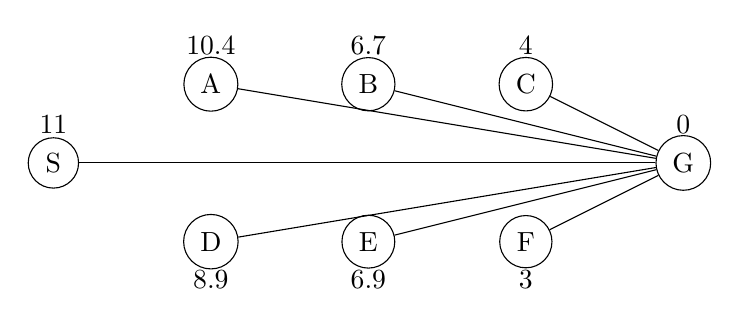
\begin{tikzpicture}
        \node [draw,circle](s)at(0,0){S};
        \node [draw,circle](a)at(2,1){A};
        \node [draw,circle](d)at(2,-1){D};
        \node [draw,circle](b)at(4,1){B};
        \node [draw,circle](e)at(4,-1){E};
        \node [draw,circle](c)at(6,1){C};
        \node [draw,circle](f)at(6,-1){F};
        \node [draw,circle](g)at(8,0){G};

        \draw (s) -- (g);
        \draw (a) -- (g);       
        \draw (d) -- (g);
        \draw (b) -- (g);
        \draw (e) -- (g);
        \draw (c) -- (g);
        \draw (f) -- (g);

        \draw (0,1/4) node[above]{$11$};
        \draw (2,5/4) node[above]{$10.4$};
        \draw (2,-5/4) node[below]{$8.9$};
        \draw (4,5/4) node[above]{$6.7$};
        \draw (4,-5/4) node[below]{$6.9$};
        \draw (6,5/4) node[above]{$4$};
        \draw (6,-5/4) node[below]{$3$};
        \draw (8,1/4) node[above]{$0$};
    \end{tikzpicture}
    \caption{Heuristic $h(n)$}
    \label{fig:greedy_search_heuristic}
\end{figure}

\noindent
However, this is not enough for optimal. We need to do something on the heuristic cost. Otherwises, the actual bad goal cost < estimated good goal cost. \textbf{Admissible heuritics} is needed, they \textbf{underestimate the actual cost}. Saying that $h$ is admissible iff for all nodes $n \le h(n) \le h^{*}(n)$ where $h^{*}(n)$ is the actual cost to the closest goal. \\
How to come up with admissible heuristics? The cost of an optimal solution to a \textbf{relaxed problem} is admissible heuristics, an understimate, for the original problem. \\
Larger admissible heuristics, better estimation, closer to actual value, \textcolor{red}{but cannot larger than actual value (upper bound).} For example, $h2$ dominates $h1$ means for all nodes $n: h2(n) \ge h1(n)$. In this case, $h2$ is always better than $h1$, but for all nodes $h1(n) \le h2(n) \le h^{*}(n)$. For two heuristics $h1$ and $h2$, $h3(n) = max(h1(n),h2(n))$ always dominates both $h1$ and $h2$, because for all nodes n, $h3(n) \ge h1(n)$ and $h3(n) \ge h1(n)$.

\subsection{UCS + Greedy Search}
\textbf{Generally, UCS + Greedy = $A^{*}$ without redundant path elimination.} For redundant paths: $A^{*}$, for memory usage $IDA^{*}.$ The properties of combination between UCS and Greedy search is shown: \\
\begin{outline}
    \1 Time complexity: $O(b^{1+\frac{C^{\prime}}{\epsilon}})$worst case $h=0$
        \2 with b: branching factor, $C^{*}$: solution cost, arc cost (cost between 2 neighbor nodes) at least $\epsilon$ shallowest-solution depth
    \1 Space complexity: $O(b^{1+\frac{C^{\prime}}{\epsilon}})$worst case $h=0$
        \2 with b: branching factor, $C^{*}$: solution cost, arc cost (cost between 2 neighbor nodes) at least $\epsilon$
    \1 Completeness: yes due to optimal
    \1 Optimal: yes, if admissible heuristics
\end{outline}

\noindent
\textcolor{orange}{\textbf{Proof of optimality of UCS + G is shown:}}
\begin{enumerate}
    \item Imagine B (suboptimal) is on the fringe
    \item Imagine some ancestor n of A (optimal) is on the fringe too
    \item n will expaned before B
    \begin{enumerate}
        \item $f(n)$ is less or equal to $f(A)$ due to admissible heuristics
        \item $f(A)$ is less or equal to $f(B)$ due to admissble heuristics
        \item n expands before B
    \end{enumerate}
    \item All ancestors of A expand before B
    \item A (optimal) expands before B (suboptimal)
    \item UCS + G search is optimal
\end{enumerate}

\subsection{Redundant Paths}
Key: failure to detect \textbf{repeated states} can cause exponentially more work. \textbf{Idea: never expand a state twice.} One way to implement is shown:
\begin{enumerate}
    \item \textbf{Keep track} of set of expanded states "closed set"
    \item Expand the search tree node-by-node
    \item Before expanding a node, \textbf{check} to make sure its state has never been expanded before
    \item \textbf{If not new, skip it, if new add to closed set.}
\end{enumerate}

\begin{figure}[htbp]
    \centering
    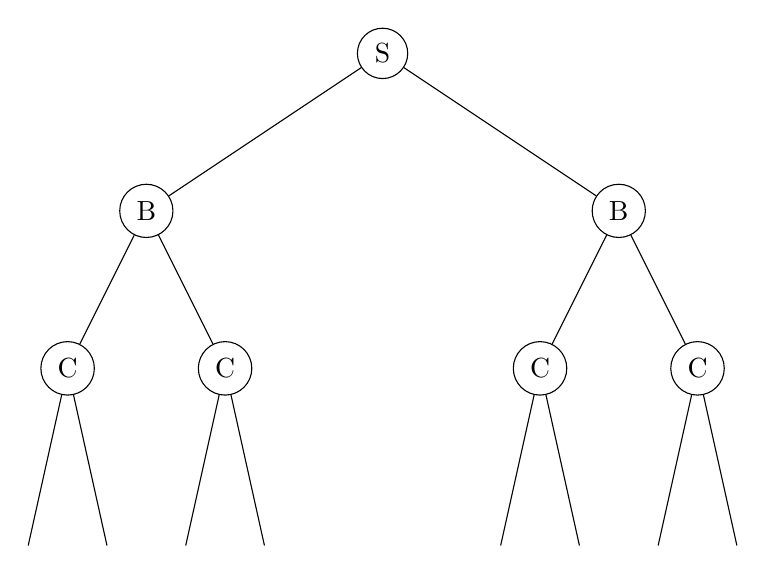
\begin{tikzpicture}
        \node [draw,circle](a)at(4,6){S};
        \node [draw,circle](b1)at(1,4){B};
        \node [draw,circle](b2)at(7,4){B};
        \node [draw,circle](c1)at(0,2){C};
        \node [draw,circle](c2)at(2,2){C};
        \node [draw,circle](c3)at(6,2){C};
        \node [draw,circle](c4)at(8,2){C};

        \draw (a) -- (b1);
        \draw (a) -- (b2);       
        \draw (b1) -- (c1);
        \draw (b1) -- (c2);
        \draw (b2) -- (c3);
        \draw (b2) -- (c4);
        \draw (c1) -- (-1/2,-1/4);
        \draw (c1) -- (1/2,-1/4);
        \draw (c2) -- (3/2,-1/4);
        \draw (c2) -- (5/2,-1/4);
        \draw (c3) -- (11/2,-1/4);
        \draw (c3) -- (13/2,-1/4);
        \draw (c4) -- (15/2,-1/4);
        \draw (c4) -- (17/2,-1/4);
    \end{tikzpicture}
    \caption{Repeated state without redundant path elimination}
    \label{fig:repeated_state_without_rpe}
\end{figure}

\noindent
Generally, 
\begin{outline}
    \1 UCS + Greedy search = $A^{*}$ without redundant path elimination
    \1 $A^{*}$ = UCS + Greedy search + redundant path elimination
\end{outline}

\noindent
The algorithm of redundant path elimination \emph{(First version: the closed set, not the path deletion version)} is shown as below: \\ \\
\textbf{Input:}
\tabto{5mm} a graph,
\tabto{5mm} a set of start nodes,
\tabto{5mm} Boolean procedure $goal(n)$ that tests if $n$ is a goal node. \\
\emph{frontier} := {$<s>$: $s$ is a start node} \\
\textcolor{red}{\emph{closed} := \{\}} \\
\textbf{while} \emph{frontier} is not empty:
\tabto{5mm} \textbf{select} and \textbf{remove} path $<n_{0},...,n_{k}>$ from \emph{frontier}
\tabto{5mm} \textcolor{red}{\textbf{if} $n_{k} \notin closed$ \textbf{then}}
\tabto{10mm} \textcolor{red}{add $n_{k}$ to \emph{closed}}
\tabto{10mm} \textbf{if} \emph{goal($n_{k}$)}
\tabto{15mm} \textbf{return} $n_{0},...,n_{k}$
\tabto{10mm} \textbf{for every} neighbor $n$ of $n_{k}$
\tabto{15mm} \textbf{add} $n_{0},...,n_{k}$ to \emph{frontier} \\
\textbf{end while} \\

\subsection{$A^{*}$ went wrong}
\noindent
Problem: When $A^{*}$ gone wrong?. If the heuristics is \textbf{\textcolor{red}{not consistent}}. There are two options: consistent heuristics or repair the frontier
\begin{enumerate}
    \item Consistent heuristics: ensure that the first "selected" path to a node always has lowest cost, thus, we can directly prune node by closed set without considering. \emph{(This can only work for consistent admissble heuristics)}
    \item Repair the frontier: if there is a path $p = <s,...,n,...,m>$ on the frontier and a path $p^{\prime}$ to $n$ such that $g(p^{\prime} \ge g(p))$ then remove $p^{\prime}$ from the frontier. \emph{(This can work for any admissible heuristics)}
\end{enumerate}

\subsubsection{Consistent heuristics}
\noindent
Difference between admissibility and consistency. But the main idea for both is "estimated heuristic cost $\le$ actual consts". Generally, \textbf{consistency $\rightarrow$ admissibility}. Consistency makes $A^{*}$ having a \textbf{f-contour}, and increase this \textbf{"f-contour"} one by one.
\begin{outline}
    \1 Admissibility: from A to G, heuristic cost $\le$ actual cost to goal (for whole)
        \2 $h(A) \le$ actual cost from A to G
    \1 Consistency: for each path from power set of from A to G, heuristic "arc" cost $\le$ actual cost for each arc
        \2 $h(A) - h(C) \le$ cost (A to C)
\end{outline}

\subsubsection{repair frontier}
For repairing the frontier, we need to compare new repeated path, and the state in the current path, the algorithm is shown as below: \textbf{(no closed set exist)} \\

\noindent
\tabto{0mm} \textbf{Input:}
\tabto{5mm} a graph,
\tabto{5mm} a set of start nodes,
\tabto{5mm} Boolean procedure $goal(n)$ that tests if $n$ is a goal node.
\tabto{0mm} \emph{frontier} := {$<s>$: $s$ is a start node}
\tabto{0mm} \textcolor{red}{\st{\emph{closed} := \{\}}}
\tabto{0mm} \textbf{while} \emph{frontier} is not empty:
\tabto{5mm} \textbf{select} and \textbf{remove} path $<n_{0},...,n_{k}>$ from \emph{frontier}
\tabto{5mm} \textcolor{red}{\st{\textbf{if} $n_{k} \notin closed$ \textbf{then}}}
\tabto{10mm} \textcolor{red}{\st{add $n_{k}$ to \emph{closed}}}
\tabto{5mm} \textcolor{blue}{\textbf{if} \emph{goal($n_{k}$)}}
\tabto{10mm} \textcolor{blue}{\textbf{return} $n_{0},...,n_{k}$}
\tabto{5mm} \textcolor{blue}{\textbf{for every} neighbor $n$ of $n_{k}$}
\tabto{10mm} \textcolor{blue}{\textbf{add} $n_{0},...,n_{k}$ to \emph{frontier}} 
\tabto{5mm} \textcolor{blue}{\textbf{if} there are $p = <s,t_{1},t_{2},...,t_{k},i,...,m>$ and $p^{\prime} = <s,s_{1},s_{2},...,s_{l},i>$ on the frontier and $g(p^{\prime}) \ge g(p)$} 
\tabto{10mm} \textcolor{blue}{\textbf{then} remove all such $p^{\prime}$} 
\tabto{0mm} \textbf{end while} \\

\subsection{Iterative Deepening $A^{*}$}
Idea from $A^{*}$ with consistent heuristics, with increasing "f-contour". Can we do this \textbf{iteratively}? Get DFS\'s space advantages with $A^{*}$ time. The difference between ID and ID$A^{*}$ is \textbf{how to choose "contour limit"}. The ID$A^{*}$ usually combined with loop breaking instead of redundant path elimination (this is not $A^{*}$), as this requires to store all generated nodes (closed set).
\begin{outline}
    \1 For ID, just do a DFS, if no solution, just limit = limit + 1
    \1 For ID$A^{*}$, if no solution, \textcolor{blue}{\textbf{use the smallest f value as the next contour.}}
\end{outline}

\noindent
The algorithm of ID$A^{*}$ is shown as below: \\ \\
\tabto{0mm} \textbf{procedure f-limited-search (}
\tabto{5mm} \textbf{input:} a graph,
\tabto{5mm} a set of start nodes,
\tabto{5mm} Boolean procedure \emph{goal(n)} that tests if \emph{n} is a goal node,
\tabto{5mm} \textcolor{red}{$f_{bound}$: positive number}
\tabto{0mm} )
\tabto{0mm} \emph{frontier} := {$<s>$: $s$ is a start node}
\tabto{0mm} $f_{next}$ := $\infty$
\tabto{0mm} \textbf{while} \emph{frontier} is not empty:
\tabto{5mm} \textbf{select} and \textbf{remove} first $p = <n_{0},...,n_{k}>$ from \emph{frontier}
\tabto{10mm} \textbf{if} $goal(n_{k})$ \textbf{then return} $p$
\tabto{10mm} \textbf{for every} neighbor $n$ of $n_{k}$
\tabto{15mm} compute $f_{n} = f(<n_{0},...,n_{k},n>)$
\tabto{15mm} \textbf{if} $f_{n} \le f_{bound}$
\tabto{20mm} \textbf{then add} $<n_{0},...,n_{k},n>$ to front of \emph{frontier}
\tabto{15mm} \textbf{if} $f_{n} > f_{found}$ and $f < f_{next}$
\tabto{20mm} \textbf{then} $f_{next} := f_{n}$
\tabto{0mm} \textbf{end while}
\tabto{0mm} \textbf{return} $f_{next}$

The properties of ID$A^{*}$ is shown as below:
\begin{outline}
    \1 Time complexity: worst case like $b^{0} + (b^{0} + b^{1}) + (b^{0} + b^{1} + b^{2}) + ... + (b^{0} + b^{1} + ... + b^{N}) = ...$, \textcolor{red}{which is $O(b^{\frac{C^{*}}{\epsilon}})$, as ID is $O(b^{d})$}
        \2 with b: branching factor, $C^{*}$: solution cost, arc cost (cost between 2 neighbor nodes) at least $\epsilon$ shallowest-solution depth, s: shallowest-solution depth
    \1 Space complexity: \textcolor{red}{$O(b \times \frac{C^{*}}{\epsilon})$ worst case $h=0$, as ID is $O(b \times s)$}
        \2 with b: branching factor, $C^{*}$: solution cost, arc cost (cost between 2 neighbor nodes) at least $\epsilon$, s: shallowest-solution depth
    \1 Completeness: yes due to optimal
    \1 Optimal: yes, under same situation as UCS + Greedy Search \emph{(Consistent admissible heuristics or redundant path elimination)}
\end{outline}


\subsection{Summary}
\begin{enumerate}
    \item The best heuristics $f(n) = g(n) + h(n)$ is an \textbf{admissble heuristics} with the combination of Uniformed Cost Search and Greedy Search.
    \item Coming up with a good admissible heuristics is important (larger -> better -> closer to the $h^{*}(n)$ (actual value), but also should be (for all nodes n) smaller than $h^{*}(n)$)
    \item \textbf{Heuristics design} is key for searching problem!
    \item Uniformed search vs. Informed Search = with or without \textbf{"heuristics"}
    \item $f(n) = g(n) + h(n)$, \textbf{difference choices $\rightarrow$ difference algorithms}, where without $g(n)$ is Greedy search, and without $h(n)$ is UCS, with both $g(n)$ and $h(n)$ is $A^{*}$ without redundant path elimination.
    \item Important \textbf{FOUR} properties for an algorithm: Time complexity, Space complexity, Completeness, Optimality.
\end{enumerate}

\pagebreak